\documentclass[10pt,a4paper]{article}
\usepackage[left=2.5cm,right=2cm]{geometry}

\usepackage[spanish]{babel}
\usepackage[T1]{fontenc}
\usepackage[utf8]{inputenc}
\usepackage{hyperref}
\usepackage{graphicx}

\title{Pan de fermentación natural}

\begin{document}
\maketitle
\tableofcontents

\section{Materieales}

\begin{itemize}
\item Levain activo
\item  Harina comun e integral (opcional recomendado la integral)
\item  Harina de centeno (opcional)
\item  Un bowl de cualquier material medio circular de uno o dos litros de tamaño, donde vamos a dejar fermentar el pan
\item  Agua mineral (opcional, podes usar de canilla o filtrada, yo uso mineral pero no debe ser relevante)
\item  Un repasador limpio, lavado sin suavizante, acá vamos a apoyar el pan,
  muy importante que no tenga olor a nada porque trasmite todo al pan y queda
  horrible. Idealmente de un color que contraste con la harina.
\item  Un horno normal hogareño que llegue a una buena temperatura, si tiene ventilador recomiendo desenchufarlo para que el viento no se lleve al vapor
\item  Una asadera
\item  Algun recipiente que resista horno para meter agua y generar vapor. No
  recomiendo vidrio o pirex, porque el shock térmico al momento de agregarle el
  agua lo puede destruir.
\item  Una gilette de las antiguas (ideal) o al menos un cuchillo bien afilado
\item  Manopla para manipular las asaderas muy calientes en el horno
\item  Idealmente un bench scrapper, una espatula grande, o una cuchilla grande
\end{itemize}

\section{Receta}
Esta es la receta que usamos durante la juntada

\url{https://bread-formula.sebastian-galkin.com/calculate?wfp=15&sp=2.1&lvp=25&lvwfp=20&td=800&hy=70&lvhy=70&dp=38}

Pueden jugar con los números y recalcular la receta.  Si guardan la URL
después de calcular, recuperan la receta.

Acuérdense que la cantidad de agua depende muchísimo del tipo de harina que
tengan (incluso hay diferencias entre dos paquetes de harina de la misma marca),
del clima, de su experiencia, etc.

\section{Levain}
\subsection*{Cuándo}
Preparar el levain como para que esté cerca del pico en el momento de amasar.
Algunas horas de diferencia no es problema, pero si esta muy joven o muy pasado,
puede tardar mucho el proceso de fermentación.

\subsection*{Por qué}
Porque un pan sin fermento queda como un ladrillo.

\subsection*{Notas}
\begin{itemize}
\item El levain tiene que estar activo y fuerte, al menos duplicar en
  volumen en menos de 24 horas.
\item Yo recomiendo levain 20\% integral y con una composición de harinas de
  20\% integral y 80\% blanca. Pero hay muchas posibilidades avanzadas para jugar.
\item En general un levain ``viejo'' te da un sabor mas ácido que uno joven.
\end{itemize}

\section{Autólisis}
\subsection*{Cuándo}
$t=0$
\subsection*{Por qué}
\begin{itemize}
\item Reduce tiempo de amasado
\item Menos trabajo
\item Menos oxidación durante el amasado $\rightarrow$ mejor sabor
\end{itemize}

\subsection*{Notas}
La autólisis es el proceso de mezclar el agua y las harinas, sin fermento ni
sal, y dejarlos reposar por un tiempo. No hace falta amasar, solo integrar los
ingredientes de forma homogénea.

\begin{itemize}
\item Mezclar las harinas bien
\item Agregar el agua, reservar 15g
\item Integrar todos los componentes hasta que quede una masa homogénea
\item No amasar
\item Dejar una hora en un bowl tapado. Si hace más de 26 grados dejar en la
  heladera. Si hace mucho calor, arrancar con agua de heladera.
\end{itemize}

La fermentación no arranca sin el fermento, pero las enzimas si.

Si leen por ahí, van a ver que hay mucha gente que dice que hace autólisis con
el fermento ya aplicado. Esa gente está equivocada.

La autólisis se puede hacer desde 20 minutos hasta 48 horas, en mi
experiencia con una hora tenés la mayoría del efecto deseado, sin
peligros de debilitar la harina.

\section{Amasado}
\subsection*{Cuándo}
Autólisis + 1 hora

\subsection*{Por qué}
El objetivo es forzar al agua en contacto con cada molécula
de harina, para activar la generación de gluten. No es fácil
llegar a todas las moléculas. La tracción talvez ayuda un poco
con el desenvolvimiento del gluten, pero todo el resto sobre alinear
las cadenas de gluten y que se yo es verso.

\subsection*{Notas}
\begin{itemize}
\item Incorporar el levain a la masa del autolize, mezclar hasta integrar
\item Incorporar la sal y mezclar hasta integrar, usar el resto del agua
  guardada para ayudar a disolver la sal.
\item Amasar: Levantar la masa de una punta, golpearla contra la mesa (suavemente),
  estirarla un poco, doblar, repetir a 90 grados.
\item Dependiendo de que tan buena sea tu técnica y que tan buena sea tu
  harina, puede llevar de 3 a 30 minutos.
\item No hace falta fuerza, mejor cambiar fuerza por velocidad
\item Cuanto menos tiempo de contacto de la masa  con los dedos,
  menos se pega, usar dedos y no palma de la mano
\item Al principio parece un engrudo horrible, pero después con
  el amasado se va despegando de la mesa y las manos
\item Es bueno ir parando para no laburar al pedo, el tiempo también ayuda.
  Amasás 3 o 4 minutos, parás 1, etc.
\item Amasar hasta estar cerca de pasar el test de ventana:
  \url{https://www.youtube.com/watch?v=hZ_Jxo8bQVk}
\item Finalizado el amasado, dejar tapado con un poquito de aceite
  en el bowl.

\end{itemize}

\section{Pliegues}
\subsection*{Cuándo}
\begin{enumerate}
\item 15 minutos después del amasado
\item 20 minutos después del anterior
\item 35 minutos después del anterior
\item 1 hora después del anterior
\item ...
\end{enumerate}

En general parar los pliegues o atrasarlos  si se ve que la masa
ya conserva la forma de los pliegues anteriores, no se ``desparrama''.

\subsection*{Por qué}
\begin{itemize}
\item El principal objetivo es ayudar a desarrollar el gluten lo que le da más
  fuerza a la masa.
\item Objetivo secundario, homogeneizar temperatura si arrancaste con agua fría.
\item El pan no puede generar burbujas nuevas, solo puede hacer crecer y
  juntar las que ya se generaron durante el amasado y los pliegues.
\end{itemize}

\subsection*{Notas}
Si no lo haces, obtenés un pan con muy pocos o ningún alveolo, y miga
generalmente medio pesada.

Los pliegues después de 2:30 o 3 horas de fermentación conviene hacerlos con
bastante delicadeza para no desperdiciar gases. Los gases que se van acumulando
en la masa son un componente muy importante del sabor, no los queremos perder.

No olvidarse de tapar el bowl después de cada pliegue.

\section{Preboleo}
\subsection*{Cuándo}
Decidir cuando la fermentación está lista es una de las partes más difíciles, y
básicamente es experiencia.

\begin{itemize}
\item La masa se siente inflada, llena de aire
\item Cuando la doblas queda un borde grueso, como si doblaras algo con relleno
\item No se pega tanto a las manos ni al bowl
\end{itemize}
\subsection*{Por qué}
El preboleo le da un ultimo golpe de fuerza a la masa para mantener la forma. Si
haces un único boleo en vez de dos, se deforma más. Si por caso de emergencia
estás medio pasado de fermentación y no te da para dos boleos, no pasa nada,
hacer solo uno.

\subsection*{Notas}
Muy poca o nada de harina en la mesa. Yo muchas veces lo hago con cero harina,
solo humedezco un poco la mesa.

El preboleo es más delicado que el boleo definitivo, la idea es acomodar un poco
la masa para que gane fuerza/forma y luego dejarla reposar para que relaje
nuevamente. No queremos perder gas al pedo.

Después de bolear dejar tapado para que no se seque.

\section{Boleo}
\subsection*{Cuándo}
15 a 20 minutos después del preboleo. Si la masa está muy hidratada se va a
relajar antes, si está más seca va a tardar un poco más.

relajar = perder forma
\subsection*{Por qué}
Este es el boleo final para darle forma antes de ir al bowl definitivo.
\subsection*{Notas}
Hay que dar forma de semiesfera, y generar tensión en la superficie superior del pan tratando de perder la menor cantidad de gas posible, con delicadeza.

Dar vuelta el pan después del preboleo, lo que estaba arriba queda abajo. Juntar
las puntas hacia el centro, dar vuelta y empezar a arrastrar en la superficie
con poquísima harina. Se arrastra para generar tensión en la superficie,
aprovechás que el pan se pega un poco a la mesa y lo vas tensionando.

Cuando ya lo tenés con forma redondeada y con suficiente tensión, levantarlo y
ponerlo con la parte de arriba (la tensionada y lisa) hacia abajo en un bowl,
sobre un trapo enharinado. Poner harina en la base del pan, tapar con el trapo y
meter en una bolsa.

\section{Retardo}
\subsection*{Cuándo}
De 0 a 30 minutos después del boleo. Es difícil saber cuando. Si lo hundís con
un dedo un poco, vuelve lentamente y tal vez no llega a recuperar totalmente su forma.
\subsection*{Por qué}
Para ganar sabor, hay mucha diferencia entre un pan con y sin
retardo, los dos están buenos, pero la diferencia se nota. La fermentación se
desacelera muchísimo, pero las enzimas siguen laburando.

\subsection*{Notas}
Meter el pan en la heladera, con la bolsa cerrada para que no pierda humedad ni
capture olores no deseados.

\section{Cocinado}
\subsection*{Cuándo}
De 12 a 24 horas después de entrar en la heladera.
\subsection*{Por qué}
D'oh!.
\subsection*{Notas}
\begin{itemize}
\item Precalentar horno una hora al mango (no se, 260 grados)
\item Precalentar junto con el horno la asadera y un recipiente para meter
  agua en el horno
\item Hervir agua
\item Cuando está caliente el horno sacar el pan de la heladera hacerle un
  corte con una gilette o cuchillo muy afilado. Hay muchos cortes posibles,
  pero en principio arranquen con un corte en un costado, de toda la
  longitud del pan, con la gilette a 30 grados de la superficie.

\item Meter el pan al horno rápidamente, tirar agua hirviendo en el
  recipiente y cerrar el horno ASAP.
\item Cocinar 17 minutos para un pan de 800 gramos de masa cruda. Luego
  retirar el agua, girar el pan y seguir cocinando por otros 15 minutos.
  Luego cocinar aproximadamente 8 o 10 minutos más, pero ir guiándose por el
  color y sonido. Si se golpea en la base, cuando está listo suena hueco.
\item Después de los primeros 17 minutos, ir girando el pan cada tanto para
  asegurarse dorado parejo si tu horno no es muy bueno.
\item Para saber si la temperatura está bien, a la hora de sacar el agua del
  horno, el pan no tiene que haber empezado a dorarse aún, o si se doró tiene
  que ser casi nada.

\end{itemize}

\section{Enfriado}
\subsection*{Cuándo}
Después de sacar del horno.
\subsection*{Por qué}
Adentro del pan hay alta temperatura y mucho vapor, el pan se sigue cocinando en
el centro mientras se enfría. Si lo cortás inmediatamente, todo ese vapor escapa
y el pan se seca un poco.
\subsection*{Notas}
No seas pelotude, con tanto laburo no te dejes vencer por la ansiedad.

\section{Corte}
\subsection*{Cuándo}
Después de esperar el enfriado.
\subsection*{Notas}
Cortar el pan es medio peligroso, he visto más de un accidente. El cuchillo se
patina en la superficie del pan que es dura y aterriza en un dedo. Conviene usar
un cuchillo grande, de dientes. Para cortarlo, recomiendo seguir los siguientes
pasos, ver imágen:
\begin{enumerate}
\item Apoyar el pan en su base y hacer un corte a la mitad, transversal al corte
  que tiene el pan.
\item Apoyar las mitades de pan con la miga hacia abajo.
\item Cortar las rebanadas con el pan en esa posición.
\end{enumerate}

\begin{figure}[h]
  \centering
  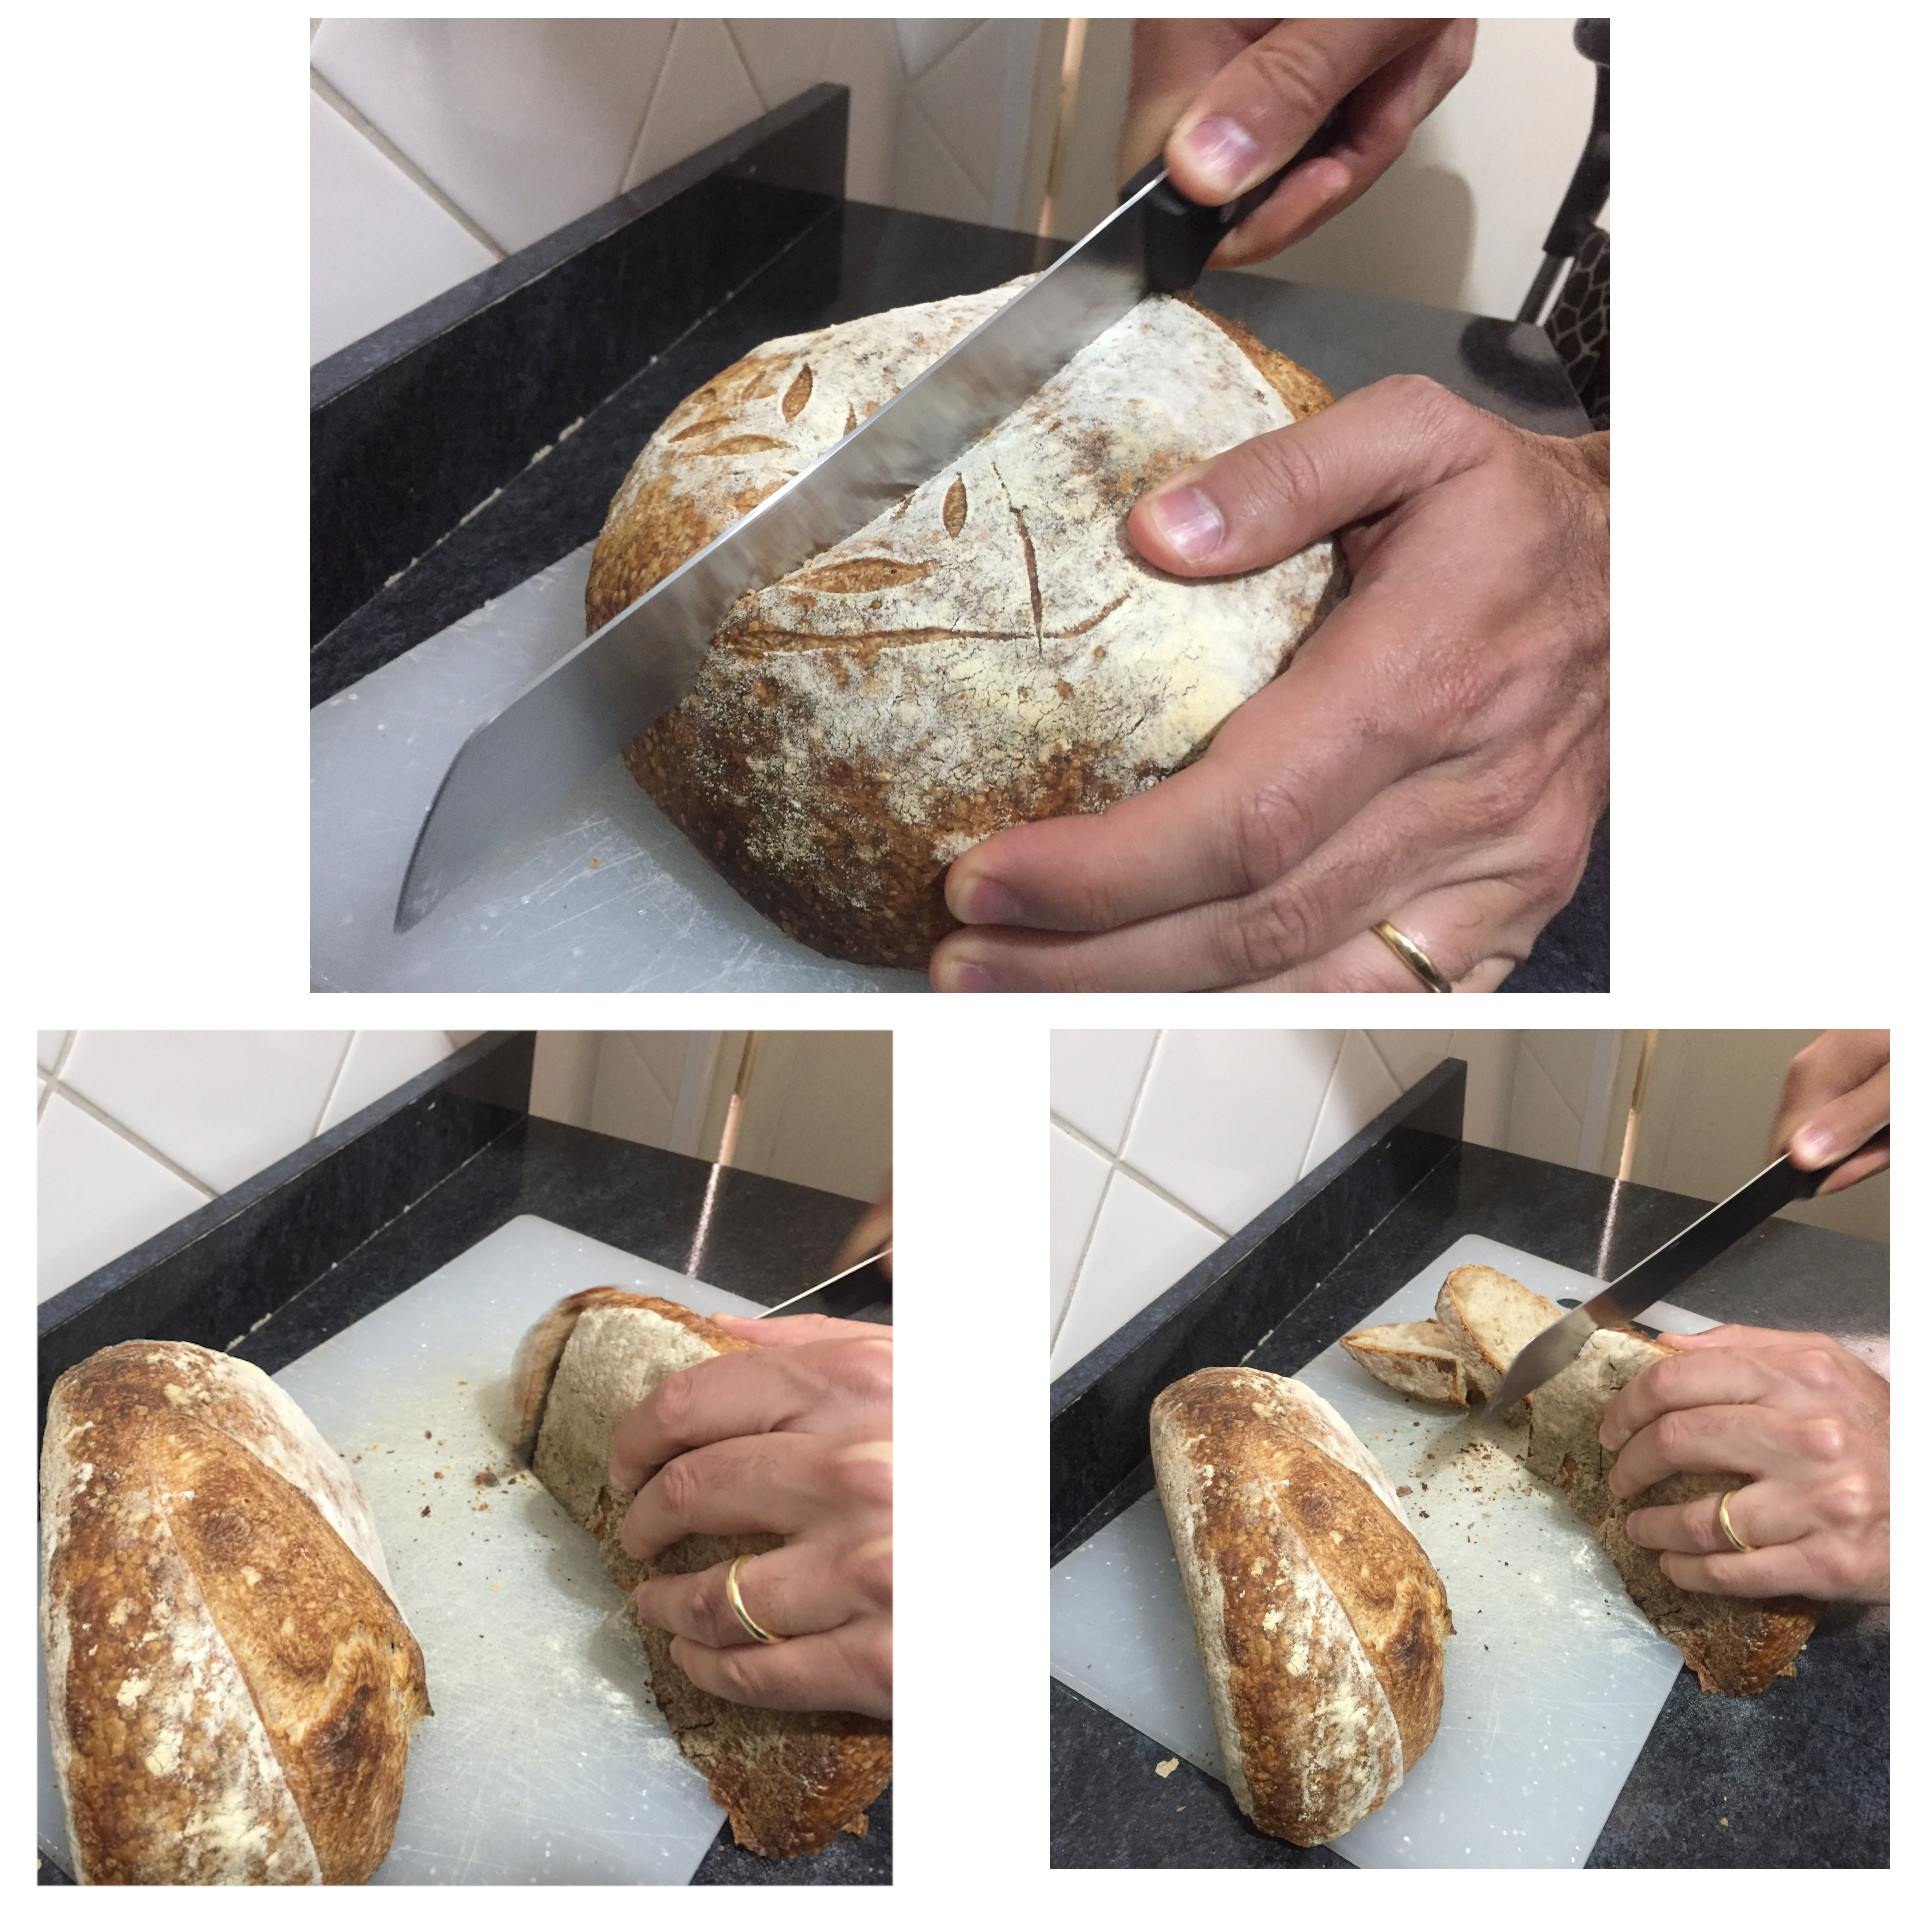
\includegraphics[width=0.8\textwidth]{cut.jpg}
\end{figure}

\end{document}